\documentclass[10pt]{article}

\usepackage[utf8]{inputenc}
\usepackage[top=2cm, bottom=2cm, left=2cm, right=2cm]{geometry}
\usepackage{color}
\usepackage[authoryear]{natbib}
\usepackage{amsmath}
\usepackage{caption}
\usepackage{subcaption}
\usepackage{siunitx}
\usepackage{setspace}
\usepackage[dvipsnames]{xcolor}
\usepackage{graphicx}
\graphicspath{ {./figs/} }

\newcounter{question}
\newcommand{\name}{00}

\renewcommand{\thefigure}{R\arabic{figure}}
\renewcommand{\thetable}{R\arabic{table}}

\newcommand{\question}[1]{\refstepcounter{question} \noindent \textbf{Comment \name.\thequestion}\vskip 0.25cm \noindent \emph{#1}\\}

\newcommand{\answer}[1]{\noindent \textbf{Answer to \name.\thequestion}\vskip 0.25cm \noindent #1 \mbox{}\\}

\newcommand{\newperson}[2]{\renewcommand{\name}{#2} \setcounter{question}{0} \noindent \textbf{\large Answers to #1} \\}

\onehalfspacing

\begin{document}

% Macros for commmon symbols <<<
\newcommand{\ypl}{y^{+}} %yPlus
\newcommand{\ured}{U^{*}} %reduced velocity
\newcommand{\yrms}{y^{*}_{\text{RMS}}} %root-mean-square of the normalised cylinder displacement
\newcommand{\ystr}{y^{*}} %the normalised cylinder displacement
\newcommand{\fstr}{f^{*}} %the normalised vibration frequency
\newcommand{\fn}{f_{n}} %system natural frequency
\newcommand{\fk}{f_{k}} %the coarsest grid in a grid independence study
\newcommand{\fvstr}{f^{*}_{v}} %normalise vortex shedding frequency
\newcommand{\fvk}{f_{v,\text{Karman}}} %Karman vortex shedding frequency
\newcommand{\fvkstr}{f^{*}_{v,\text{Karman}}} %normalised Karman vortex shedding frequency
\newcommand{\fcyl}{f_{\text{cyl.}}} %frequency of cylinder vibration
\newcommand{\fosc}{f_{\text{osc.}}} %frequency of cylinder oscillation
\newcommand{\fclstr}{f_{\text{Cl}}^{*}} %normalised frequency of lift coefficient
\newcommand{\flrms}{F_{\text{L,RMS}}} %root-mean-square of the lift force
\newcommand{\fl}{F_{\text{L}}} %the lift force
\newcommand{\clrms}{\text{Cl}_{\text{RMS}}} %root-mean-square of the lift coefficient
\newcommand{\cflyt}{C_{F_{L},y(t)}} %IMF component of lift that is most similar to the displacement signal in terms of temporal evolution of amplitude and frequency, differing only perhaps in phase OR the component of lift with the highest correlation to the displacement signal
\newcommand{\cflkrms}{C_{F_{L},\text{Karman},\text{RMS}}} %the Karman component of lift
\newcommand{\cflsrms}{C_{F_{L},\text{streamwise},\text{RMS}}} %the streamwise component of lift
\newcommand{\ccli}{C_{\text{Cl},i}} %the ith component of lift coefficient
\newcommand{\cclystr}{C_{\text{Cl},\ystr}} %the ith component of lift coefficient
\newcommand{\cflm}{C_{F_{L},\text{max}}} %IMF component of lift that has maximum RMS amplitude in the IMF set
\newcommand{\cyrms}{C_{y,\text{RMS}}} %the RMS of the component of lift that is most correlated with the cylinder displacement signal
\newcommand{\cclrms}{C_{\text{Cl},\text{RMS}}} %the RMS of the component of lift that is most correlated with the cylinder displacement signal (new symbol)
\newcommand{\cysys}{C_{\ystr,\ystr}} %the characteristic IMF representing the normalised cylinder displacement
\newcommand{\cclys}{C_{\text{Cl},\ystr}} %the characteristic IMF representing the lift coefficient
\newcommand{\afl}{\alpha_{F_{L}}} %ratio between two dominant IMF components of the lift

% Turbulence modelling related symbols
\newcommand{\nut}{\nu_{T}} %nut
\newcommand{\nuTilda}{\tilde{\nu}} %nuTilda

% Common angles
\newcommand{\angfi}{\SI{90}{\degree}} %90 deg. angle
\newcommand{\angfo}{\SI{67.5}{\degree}} %67.5 deg. angle
\newcommand{\angth}{\SI{45}{\degree}} %45 deg. angle
\newcommand{\angtw}{\SI{22.5}{\degree}} %22.5 deg. angle
\newcommand{\angon}{\SI{0}{\degree}} %0 deg. angle

\newcommand{\pfrms}{P_{\text{Fluid,RMS}}} %estimated root-mean-square of fluid power
\newcommand{\pmrms}{P_{\text{Mech.,RMS}}} %estimated root-mean-square of mechanical power
\newcommand{\etamech}{\eta_{\text{Mech.}}} %mechanical power efficiency
\newcommand{\re}{\text{Re}} %Reynolds number
\newcommand{\st}{\text{St}} %Strouhal number
\newcommand{\plag}{\theta_{y-\text{Cl}}} %Characteristic phase lag
\newcommand{\phim}{\phi_{\text{mean}}} %mean phase lag
\newcommand{\wcl}{W_{\text{cyl.}}} %mean work done by cylinder over one cycle of vibration
\newcommand{\tosc}{T_{\text{osc.}}} %mean period of cylinder oscillation
\newcommand{\meff}{m_{\text{eff.}}} %effective mass
\newcommand{\zetatot}{\zeta_{tot.}} %total damping of the system

%Macros that are shorthands in writing
\newcommand{\rms}{root-mean-square} %shorthand for root-mean-square

%Macros used in writing section on GCI study
\newcommand{\rp}{r^{p}} %refinement ratio, used in GCI study
\newcommand{\fre}{f_{\text{RE}}} %Richardson extrapolation of quantity of interest, used in GCI study

%The macros for freestream velocities
\newcommand{\uon}{\SI[per-mode=symbol]{0.1}{\metre\per\second}}
\newcommand{\utw}{\SI[per-mode=symbol]{0.2}{\metre\per\second}}
\newcommand{\uth}{\SI[per-mode=symbol]{0.3}{\metre\per\second}}
\newcommand{\ufo}{\SI[per-mode=symbol]{0.4}{\metre\per\second}}
\newcommand{\ufi}{\SI[per-mode=symbol]{0.5}{\metre\per\second}}
\newcommand{\usi}{\SI[per-mode=symbol]{0.6}{\metre\per\second}}
\newcommand{\use}{\SI[per-mode=symbol]{0.7}{\metre\per\second}}
\newcommand{\uei}{\SI[per-mode=symbol]{0.8}{\metre\per\second}}
\newcommand{\uni}{\SI[per-mode=symbol]{0.9}{\metre\per\second}}
\newcommand{\ute}{\SI[per-mode=symbol]{1.0}{\metre\per\second}}
\newcommand{\uel}{\SI[per-mode=symbol]{1.1}{\metre\per\second}}
\newcommand{\utv}{\SI[per-mode=symbol]{1.2}{\metre\per\second}}
\newcommand{\utt}{\SI[per-mode=symbol]{1.3}{\metre\per\second}}

\newcommand{\uron}{2.3}
\newcommand{\urtw}{4.5}
\newcommand{\urth}{6.8}
\newcommand{\urfo}{9.1}
\newcommand{\urfi}{11.4}
\newcommand{\ursi}{13.6}
\newcommand{\urse}{15.9}
\newcommand{\urei}{18.2}
\newcommand{\urni}{20.5}
\newcommand{\urte}{22.7}
\newcommand{\urel}{25.0}
\newcommand{\urtv}{27.3}
\newcommand{\urtt}{29.5}
% >>>
% Opening remarks <<<
\noindent {\Large \textbf{Response to the reviewers for paper OE-D20-01516: \emph{Evolution of Lift in a Pure Cruciform for Energy Harvesting}}}\\

\noindent We would like to express our gratitude to the anonymous reviewers for their time and insight. Below, we document the comments from the reviewers and our response to the comments. We indicate the changes in the original manuscript using the colour \textcolor{blue}{blue}.

\vspace{1cm}

% \newperson{Associate Editor}{AE}
% 
% \question{Question}
% 
% \answer{Answer}
% >>>
% Reviewer 1 <<<
\newperson{Reviewer 1}{R1}

\question{Why OpenFOAM is employed? If other software can be employed to solve the calculation?} \label{quest:whyOF}

\answer{
  In our opinion, any CFD software can be employed by a proficient enough user as a means to gain important insight on a subject of study. A numerical study in the area of fluid mechanics, as in other disciplines, can be of differing levels of complexity. Some are meant to be instructional, and these deal with relatively idealised cases, especially in a classroom setting. However, in a post-graduate or industrial setting, we think it is in the interest of the researcher(s) that the tool chosen to execute the numerical study fulfill the following criteria.

    \begin{enumerate}
        \item The algorithm required to carry out the numerical work must be built into the software. Else, the software itself must be easily extensible to include the numerical routine required. \label{enum:extensible}
        \item A high degree of automation must be possible on any aspect of the numerical work, be it meshing, running and control of the simulation, data collection and parameter variation. \label{enum:automation}
        \item Parallellisation is built in to the software. \label{enum:parallellisation}
        \item A stable software code base. \label{enum:stability}
        \item The software allows real-time collaboration with multiple authors across a common platform, allowing each iteration of the project or parts of it to be version controlled. \label{enum:collaboration}
        \item Cost-effective. \label{enum:cost}
    \end{enumerate}

    OpenFOAM, which at the most fundamental level is a collection of C++ library, is easily modified and extended (point \ref{enum:extensible}) using nothing more than a plain text editor, and then recompiled to include the required functionality. The use of extensible text editors such as VIM or Emacs greatly facilitates this process, and at zero cost.

    Any aspect of the workflow using OpenFOAM can be automated (point \ref{enum:automation}) through the use of PyFOAM, a Python library that allows fine-grain control of virtually every aspect of the simulation. In addition to automating the grid independency study and parameter variation, PyFOAM can also be used to post-process data by exploiting the NumPy Python library. Furthermore, parallellisation is built into the OpenFOAM code (point \ref{enum:parallellisation}), and the fact that the code is open source, facilitates the discovery and patching of bugs (point \ref{enum:stability}).

    Usage of the OpenFOAM software involves including and modifying configuration files, written as plain text files. As such, one can easily leverage the pre-existing tools used by software engineers such as Git, enabling real-time collaboration (point \ref{enum:collaboration}) between project members and provide much-needed version control of the whole project. We would like to point out all the tools mentioned in the previous discussion are available for free, incurring zero extra cost on the team, which can be beneficial especially for new and emerging laboratories, where procurement of hardwares is of higher priority.
}

\question{
    Mesh independence test is carried out using GCI method, but I think the reference can be updated. For example:[Applied Thermal Engineering. 2020;171:115090], [https://doi.org/10.1016/j.energy.
    2020.118690].
}

\answer{
  Following the suggestion from the reviewer, we added the following sentence in page 10, lines 6-9 of the revised manuscript.

  \begin{quotation}
    \color{blue}
    \noindent A common method for checking the grid independency of quantities of interest in a numerical study is by demonstrating that one obtained similar results on all variants of the spatial discretisation (usually three grids), and then proceeding with the numerical study using the medium variant on the computational domain (see e.g., \citet{Ding2013}, \citet{Ding2019}, or \citet{Wang2020}, who settled on the coarse variant of their spatial discretisation).
    \color{black}
  \end{quotation}
}

\question{Some figures' resolution need to be adjusted.}

\answer{
We re-exported the figures used in the revised manuscript directly into the PDF format instead of the PNG format used previously, for better resolution as per the suggestion of the reviewer.
}

\question{Boundary conditions need to be shown.} \label{q:boundConds}

\answer{
  In the revised manuscript, we included the boundary conditions in page 5, Table 1, and added the description of Table 1 in page 4, lines 11-13 as follows.

  \begin{quotation}
    \color{blue}
    \noindent Table 1 summarises the boundary conditions imposed on each of the boundary patches in the simulation domain (see Fig. 6). The symbols $U$, $p$, $\nut$, and $\nuTilda$ refer to the flow velocity, pressure, kinetic eddy viscosity and its mediating variable, respectively. At the inlet, the \texttt{fixedValue} for $U$ is the freestream velocity $U_{\infty}$ (\si[per-mode=symbol]{\metre\per\second}), while $U = \SI[per-mode=symbol]{0}{\metre\per\second}$ at the strip plate. The \texttt{fixedValue} for $p$ at the outlet is \SI[per-mode=symbol]{0}{\square\metre\per\square\second}, and the \texttt{fixedValue} for $\nuTilda$ is \SI[per-mode=symbol]{0}{\square\metre\per\second} at the cylinder and strip plate patches.
  \end{quotation}

  \color{black}
}
% >>>
% Reviewer 2 <<<
\newpage
\newperson{Reviewer 2}{R2}

\question{It's suggested to define FIM in line 37 of page 3 (sub-section 2.1), even though it's easy to know that FIM means flow-induced motion.}

\answer{We have added the definition of FIM, which is flow-induced motion, in page 3, line 16 of the revised manuscript following the suggestion by the reviewer.}

\question{Why chose the distance of $7.5D$ from front/back boundary to centre of cylinder (Fig 2)? And how did the boundary condition set in this study?}

\answer{
  We considered a few factors in determining the spanwise dimension of the simulation domain, and they fall in one of the following two categories. First, adherence to the physical manifestation of streamwise vortex shedding, as observed in experimental studies. Under this category, we note the minimum spanwise half-length of a system that required for the expression of streamwise vortex-induced vibration (SVIV) is between $2D$ to $3.2D$ (e.g., \citet{Shirakashi2001} and \citet{Koide2006}). Taking this into consideration, we doubled the length of the latter, obtaining $3.2D \times 2 = 6.4D$, and then applying a safety factor of approximately 1.2, or exactly 1.17875, arriving at a round number of $15D$ for the total spanwise length of the simulation domain, and $15D/2 = 7.5D$ as its half-length.

  The second category involves evaluating the actual implementation of spanwise lengths in similar numerical studies of SVIV. Numerical studies of SVIV, or simply the numerical study of streamwise vortex shedding from a cruciform stucture are relatively few and far between. This is probably due to the irreducibility of the SVIV phenomenon to a two-dimensional (2D) problem, which renders it more computationally demanding than the numerical study of Karman vortices shedding and by extension, Karman vortex-induced vibration (KVIV). Here, we shall discuss the spanwise lengths implemented in the handful of numerical work on SVIV and how they influece our choice of spanwise length in the manuscript.

  The earliest numerical work on SVIV from a cruciform system that we know of is the study by \citet{Deng2007}. In the paper, the authors used a spanwise length of $12D$ and identified different vibration responses of the cruciform according to the spacing of the upstream and downstream cylinders. Fast forward about a decade and we find the study by \citet{Hemsuwan2018a}, which has an equivalent spanwise length of $13D$, in \citet{Hemsuwan2018b} with an equivalent spanwise length of $14.5D$ and in \citet{Hemsuwan2018c} with an equivalent length of $16D$. All of the studies mentioned deal with cruciform systems that elicit motion of the upstream cylinder resulting from the shedding of streamwise vortices. As such, it became apparent to us that our choice of domain spanwise length, $15D$, is well within the trend found in comparable literature, which lies between $12D$ and $16D$, providing further basis to our decision.

  There is one case \citep{Zhao2018a} in which the authors implemented a spanwise length of $42D$ in their computational domain. This particular study, however, is limited to a fixed cruciform in which both of the cylinders forming the cruciform are fixed. In our opinion, by limiting their scope to a fixed cruciform, the authors of \citet{Zhao2018a} significantly eased their computational requirements - permitting them to implement a larger spanwise dimension compared to us, or the other studies we have discussed.

  As for the boundary conditions, we refer the reviewer to our reply to comment \ref{q:boundConds} of reviewer 1.
}

\question{It's suggested to presented or validated the time step (or nondimensionalised time step) of the simulation in this work.}

\answer{
In this work, we used the Courant–Friedrichs–Lewy (CFL) number as the basis for our choice of time step implemented in the simulation. The CFL number is of course defined as

\begin{equation}
  C = \frac{U \Delta t}{\Delta x},
  \label{eq:cflNo}
\end{equation}

\noindent where $C$ is the CFL number, $U$ the flow velocity, $\Delta t$ the time step and $\Delta x$ the length a cell in the discretised domain, respectively. The time step $\Delta t$ is chosen such that the condition $C < 1$ is always satisfied everywhere in the computational domain. Following the suggestion by the reviewer, we have added the following sentences through page 14, line 4 and page 15, lines 1-3 of the revised manuscript.

\begin{quotation}
  \color{blue}
  \noindent As for the temporal discretisation, we relied on a simple CFL number-based scheme \citep{Hemsuwan2018a,Hemsuwan2018b,Hemsuwan2018c}, in which the time step is chosen such that the maximum CFL number $C$ in the computational domain is always less than 1. The CFL number $C$, is defined in Eq. \ref{eq:cflNoMan} as

  \begin{equation}
    C = \frac{U \Delta t}{\Delta x},
    \tag{21} \label{eq:cflNoMan}
  \end{equation}

  \noindent where $U$, $\Delta t$ and $\Delta x$ represents the flow velocity, time step and characteristic length of cell, respectively.
  \color{black}
\end{quotation}

}

\question{In line 30 of page 15, why the sudden jump followed by a gradual drop and a gradual rise in $\yrms$ can be observed in this study but not in woks of \citet{Nguyen2012} nor \citet{Koide2013}? Any difference of parameters leads to the different results?} \label{qrevtw:jumpDrop}

\answer{
  A review of the literature on streamwise vortex shedding, with a particular focus on discussions about the degree of generated disturbance in the flow, or the level of flow turbulence, reveals three important takeaways.

  \begin{enumerate}
    \item The onset of streamwise vortex shedding brings with it an increased level of turbulence in the flow. This increases the uncertainty in the measurement of the \rms{} value of normalised vibration amplitude $\yrms$ \citep{Shirakashi1989,Zhao2018a}.
    \item The level of turbulence generated  in the flow following the onset of streamwise vortex shedding is higher when the cruciform is comprised of an upstream circular cylinder and downstream strip plate, in contrast to a cruciform made of two circular cylinders. This is evidenced by the broader distribution of cruciform downstream velocity fluctuation frequencies in the frequency domain \citep{Kato2006,Kato2012}, and also flow visualisations \citep{Kato2012,Koide2017}.
    \item In a cruciform system whose constituents are an upstream circular cylinder and a downstream strip plate, systems whose plate width to cylinder diameter ratio is equal to unity, $W = w/D = 1$, generates a higher level of turbulence compared to cruciforms with $W < 1$ \citep{Kato2012}.
  \end{enumerate}

  The turbulence intensity in our simulations is set to 5\%, to recreate the ambient flow conditions our experimental setup is exposed to. This level of 5\% is comparatively high, considering that the studies we used to benchmark our results operate in water tunnels with a turbulence level that is at 2.8\% maximum \citep{Nguyen2012,Koide2013}. Add this to the fact that we are using a 

  \begin{enumerate}
    \item circular cylinder-strip plate cruciform, and,
    \item the $W = w/D$ for our strip plate is $W = 1$,
  \end{enumerate}

  \noindent the level of turbulence in the flow, and the level of disturbance/noise resulting from it becomes an increasingly important factor in determining the evolution of the dominant flow structures, and the resulting cylinder amplitude response. The jump-drop-rise pattern observed in the amplitude responses of both our experimental and numerical work is, in our opinion, the result of an interplay between the level of disturbance/noise due to increasingly turbulent flow conditions and the ability of the streamwise vortex to withstand said disturbance. As we have alluded to in the manuscript,

  \begin{quotation}
    \noindent {\Large \textbf{``}} We, therefore, attribute this difference to the higher turbulence level set in our work. The turbulence level in the works of \citet{Nguyen2012}, for example, was  $<2.8\%$ throughout their range of Reynolds number. Instead, the initial turbulence level in our setup, both experimental and numerical, is approximately double that value. Because of this, the turbulence amplification due to the onset of streamwise vortices  \citep{Zhao2018a} - especially for a circular cylinder-strip plate cruciform \citep{Koide2017} - is also higher compared to the experiments of \citet{Nguyen2012} and \citet{Koide2013}. This higher compound turbulence warps the dominant vortical structure and introduces an increasing amount of intermittency to the lift signal, and by extension, to the displacement time history of the cylinder. {\Large \textbf{''}}
   \end{quotation}

   \noindent In our opinion, the interplay between the level of disturbance in the flow and the streamwise vortices goes as follows.

   \begin{itemize}
     \item \textbf{\textit{Sudden jump:}} At the onset of SVIV, the level of disturbance is still relatively small as the system has just barely entered the streamwise vortex shedding regime. This occurs at $\ured = \urei$, where the vortical structures are the least deformed, and because of that, the net lift driving the vibration is higher compared to when the level of flow disturbance starts to grow.
     \item \textbf{\textit{Gradual drop:}} As we increase $\ured$, the level of disturbance in the flow brought about by the rising turbulence increasingly warps the streamwise vortical structures, imparting a growing degree of intermittency on the lift and hence cylinder displacement signal ($\urni \leq \ured \leq \urte$). An increased intermittency in the cylinder displacement signal lowers its mean amplitude, which in this work is computed as $\yrms$.
     \item \textbf{\textit{Gradual rise:}} As we advance further into the SVIV regime ($\ured > \urte$), the streamwise vortices becomes even more energised and increasingly resilient to ambient disturbance. This results in a less intermittent lift, the effect of which is imparted on the cylinder displacement signal, shown in Fig. 11(b) of the revised manuscript.
   \end{itemize}

   \noindent We acknowledge a lack of explanation on this matter in the original manuscript, and have therefore included the following sentences in page 17, lines 6-7 of the revised manuscript.

   \begin{quotation}
     \color{blue}
     \noindent An intermittent lift signal imposes the same trend on the $\ystr(t)$ signal, reducing its overall mean amplitude, which we compute in this work as $\yrms$.
     \color{black}
   \end{quotation}

   \noindent and page 17, lines 12-14 of the revised manuscript,
   
   \begin{quotation}
     \color{blue}
     \noindent We interpret this as the vortical structures becoming more energised and resilient against ambient excitation the further we advance into the SVIV regime.
     \color{black}
   \end{quotation}
}

\question{The CFD over predict the frequency response and the value of St in low reduced velocity range (Fig 10), is this caused by the boundary condition or the size of computational domain?}

\answer{
  In the original manuscript, we explained the discrepancy highlighted by the reviewer as follows.

  \begin{quotation}
    \noindent {\Large \textbf{``}} The discrepancies found especially in Fig. 10b most probably stem from the same reasons explained by \citet{Nguyen2012}. The lowest  $\yrms$ recorded in our simulation within  $\urth \leq \ured \leq \ursi$ was in the order of $10^{-5}$ \si{\metre} (10 microns). A numerical study has no problem recording vibration of this order as the precision of the numerical solution is only limited by the processor architecture. Experimental work, however, requires not only the sensitivity but also the isolation from the background noise that forces the cylinder to vibrate close to the natural frequency of the system  $\fn$ \citep{Nguyen2012}, which consequently overpowers this minimal amplitude vibration. Once streamwise vortices form, however, their shedding and cylinder vibration synchronises close to $\fn$, thus locking the normalised vibration frequency back to  $\fstr \approx 1$. {\Large \textbf{''}}
  \end{quotation}

  Recall that the frequency overshoot occurs within a range of $\ured$ where the vibration amplitude of the cylinder is especially small. In fact, this region of especially small vibration amplitude - in the order of 10 microns in our simulation - has been reported by \citet{Nguyen2012} and \citet{Nguyen2010} as the region where selective resonance takes place (see, e.g., \S4.3 of \citet{Nguyen2010} and \S4.3 of \citet{Nguyen2012}). When said selective resonance takes place, the randomly appearing external excitation causes the frequency spectra of the cylinder displacement to register a frequency close to the natural frequency of the system $\fn$ - in other words, $\fstr \approx 1$ - as the dominant frequency, overpowering the actual frequency at which the cylinder vibrates. In our humble understanding of their work, \citet{Nguyen2010} and \citet{Nguyen2012} simply excluded the data points that results from the selective resonance - all of which are close to $\fn$ - from their frequency response plot. We provide the original quote from \S4.3 of \citet{Nguyen2012} below.

  \begin{quotation}
    {\Large \textbf{``}} It is noted that when the oscillation amplitude is small in air flow, the spectrum of displacement, $S_{z}$, has a peak at $\fn$, in addition to $f_{v}$, due to the selective resonance which commonly occurs for a low-damped system exerted by alternating force having broadly distributing spectrum as shown in Fig. 4. In Fig. 7, and in the following figures in this paper, such data for $f_{z}$ are not plotted. {\Large \textbf{''}}
  \end{quotation}

  We decided to adopt a different approach and reported our experimental results as-is, including those affected by the selective resonance. This is why our experimental measurement of $\fstr$ returns a value close to 1 within $\urth \leq \ured \leq \ursi$. However, numerical studies are immune from the random external excitations that experimental investigations are subject to, unless they are explicitly defined in the numerical setup. Therefore, the overshot values of $\fstr$ are in our humble opinion the limit to which $\fstr$ will approach as random, external perturbations on the flow approaches zero.

  Acknowledging the inadequacy of our explanation in the original manuscript, we added the following sentence in the revised version.

  \begin{quotation}
    \color{blue}
    \noindent The values of $\fstr$ between $\urth \leq \ured \leq \ursi$ can therefore be considered as the limit of $\fstr$ in that range of $\ured$, which is appoached as the random background forcing present in experimental works tend to zero.
    \color{black}
  \end{quotation}

}

\question{It's interested that the fluctuation exists in Fig 11(a) when $\ured = \urte$, how this exist and how the value of $\yrms$ and $\fstr$ calculated for this case (The values can be found in Fig 10)?}

\answer{
  \hspace*{-0.3cm} The fluctuations that exist at $\ured = \urte$ are the direct result of the vortex structure - turbulence level interplay mechanism explained in the answer for question \ref{qrevtw:jumpDrop}.

  We compute the \rms{} value of a given quantity using the formula in Eq. \ref{eq:rmsDiscretised}.

  \begin{equation}
    \yrms = \frac{1}{N} \sqrt{\sum_{i = 1}^{i = N} \left( \ystr_{i} \right) ^{2}}.
    \label{eq:rmsDiscretised}
  \end{equation}

  \noindent Here, $N$ is the total number of data points, and $\ystr$, the normalised cylinder displacement value. Equation \ref{eq:rmsDiscretised} is used to compute the values of $\yrms$ at all $\ured$, including at $\ured = \urte$.

  We compute the values for $\fstr$ by performing the ensemble empirical mode decomposition (EEMD) on the normalised cylinder displacement signal $\ystr$. Then, we take the component with the largest \rms{} amplitude and compute its Hilbert transform, giving us the instantaneous frequency, a quantity that is a function of time. Finally, we compute the mean of that instantaneous frequency signal, giving us the characteristic frequency of $\ystr$, designated as $f$. Normalising $f$ with $\fn$ gives us $\fstr$. The values of $\fstr$ at all $\ured$ are computed using this method, including that at $\ured = \urte$. The values of $\fstr$ can also be computed via fast Fourier transform (FFT), yielding similar results.

  The reason we opted for the method above to compute $\fstr$ is because we are able to obtain the instantaneous frequency signal of $\ystr$ during the process of computing phase lag between $\ystr$ and $\fstr$, which greatly steamlines our simulation post-processing, instead of running the results separately through FFT for the sole purpose of estimating $\fstr$. To highlight this point, we included the following sentence in page 18, lines 3-5 of our revised manuscript.
  
  \begin{quotation}
    \color{blue}
    \noindent Here, $\fstr$ is computed as the mean instantaneous frequency of the dominant component of $\ystr$, which we obtain in the course of calculating the phase lag between $\ystr$ and lift. The procedure employed to decompose the $\ystr$ signal and obtain the instantaneous frequency is elaborated in \S5.1.
    \color{black}
  \end{quotation}
}

\question{Looks like that the values still going to decline in Fig 12(a). It means that the vibration here still doesn't stable?}

\answer{
  The $\ystr$ and Cl signals presented in Fig. 12(a) are the results at $\ured = \urtw$, and at $\ured = \urtw$, the cylinder vibration is in the initial branch of KVIV. Among the vibration characteristics of a VIV oscillator in the initial branch is its quasi-periodic nature \citep{Khalak1999}, which implies a modulated vibration amplitude along the time axis, where it increases and decreases cyclically. This is most simply demonstrated through a full flow time visualisation of $\ystr$ at $\ured = \urtw$, shown in Fig. 1, which bears striking resemblance to Fig. 15 of \citep{Khalak1999}.

  \begin{figure}[htpb]
    \centering
    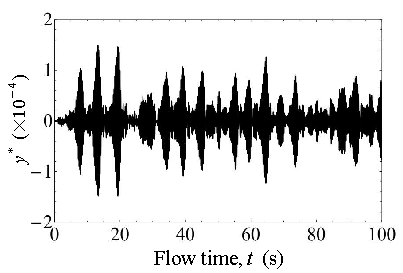
\includegraphics{ystrU02Full}
    \caption*{Figure 1: Full flow time visualisation of $\ystr$ at $\ured = \urtw$}
  \end{figure} \label{fig:fullFlowtimeU02}

  Our choice of omitting the full flow time in our Hilbert-Huang transform (HHT) analysis is because the pre-processing algorithm EEMD is computationally expensive \citep{Lv2019,Shifat2020}, and we therefore limit ourselves only to a subset of the data instead.
}

\question{How it's possible that $\pfrms < \pmrms$ for a given reduced velocity (Fig 20)?}

\answer{
  Unlike the equation to compute fluid power, shown in Eq. \ref{eq:rmsFluidPower},

  \begin{equation}
    \pfrms = \frac{1}{2} \rho \pi \cclrms U^{2} \fcyl \yrms D L \sin(\phi),
    \label{eq:rmsFluidPower}
  \end{equation}

  \noindent the original form of the equation in \citet{Raghavan2007} used what basically amounts to maximum lift amplitude $C_{y}$ in place of $\cclrms$, and the maximum cylinder displacement amplitude $y_{\text{max.}}$ in place of $\yrms$.

  As mentioned in the original manuscript,

  \begin{quotation}
    {\Large \textbf{``}} We use $\cclys$ to represent $\cclrms$ in Eq. 26. We choose to use \rms{} (parameters with subscript RMS) quantities in Eq. 25 instead of the maximum values like the original authors because that may lead to a misunderstanding that the maximum value is sustained throughout the observation window. {\Large \textbf{''}}
  \end{quotation}

  \noindent Therefore, $\pfrms$ as defined in Eq. \ref{eq:rmsFluidPower} estimates the \rms{} power obtainable from the streamwise component of lift alone, and not the total lift acting on the cylinder. This means that $\pfrms$ will only be approximately equal to $\pmrms$ if $\cclrms$ is the dominant component of the total lift \textbf{\textit{and}} the phase lag $\phi$ is close to \SI{90}{\degree}. The observation $\pfrms < \pmrms$ made by the reviewer simply means that these conditions are not satisfied.
}

\question{The fluid power is possible to improve by redirect the energy from the Karman to the streamwise vortex, and how it realizes? It's suggested to clarify a possible measure for it, or try to put forward an example.}

\answer{
  In the SVIV regime, the energy carried by the freestream is converted into three components, namely,

  \begin{enumerate}
    \item the generation of turbulence,
    \item the production of streamwise vortices, and
    \item the generation of Karman vortices.
  \end{enumerate}

  \noindent In other words,

  \begin{equation}
    \text{Freestream energy} = \text{Turbulence} + \text{Streamwise vortices} + \text{Karman vortices}.
    \label{eq:freesteamEnergy}
  \end{equation}
  
  \noindent To improve the power output of a cruciform energy harvester in the SVIV regime, the basic idea is to maximise the conversion of freestream energy into streamwise vortices, amplifying the \rms{} amplitude of the streamwise component of lift. One possible method to achieve this is by modifying the strip plate, which essentially is a passive downstream control mechanism, in a manner that enforces the dominance of the vortical structure that is able to lock into the natural frequency of the system $\fn$. This will lead to a larger $\cclys$, $\cysys$, and ultimately $\pfrms$ and $\pmrms$. This is the subject of our next publication. However, following the suggestion of the reviewer, we deleted the following sentence,


  \begin{quotation}
    {\Large \textbf{``}} We shall detail in our future work, a method to modulate the dominant vortical structures to achieve such a goal. {\Large \textbf{''}}
  \end{quotation}

  \noindent and included the following sentences in its place.

  \begin{quotation}
    \color{blue}
    \noindent One possible method of improving $\pfrms$ is by implementing a modified version of the cruciform that is able to enforce the dominance of the vortical structure that is able to lock into $\fn$ - which in Fig. 22 is the streamwise vortex - against the vortical structures that do not, i.e., the Karman vortices. We will outline such a method in our future work.
  \end{quotation}
  \color{black}
}
% \newperson{Reviewer 3}{R3}
% 
% \question{Question}
% 
% \answer{Answer}
% >>>
\newpage
\bibliographystyle{cas-model2-names}
\bibliography{references}

\end{document}
